\textbf{\underline{\large{1.8: Related Rates}}} \par

In this course, derivatives have primarily been interpreted as the slope of the tangent line. But, as with \href{https://www.merriam-webster.com/dictionary/rectilinear\%20motion}{\text{\textcolor{blue}{rectilinear motion}}}, there are other contexts for the derivative. One overarching concept is that the derivative is a \textbf{rate of change}. The tendency is to think of rates as distance per time unit, like miles per hour or meters per second, but even slope is a rate of change---it is just that the rise and run are both measured as distances. \par

The idea behind related rates is two-fold. First, change is occurring in two or more measurements that are related to each other by the geometry (or algebra) of the situation. Second, an implicit Chain Rule situation exists in that the $x$ and $y$-values are functions of time, which may or may not be a variable in the problem. Therefore, when taking the derivative of an $x$ or $y$, an \textbf{implicit rate term} $\left(\dfrac{dx}{dx} \text{ or } \dfrac{dy}{dt}\right) \forcespace$ often occurs. \par

\begin{tcolorbox}[objective]
    \begin{center}
        OBJECTIVES \\[11pt]
    \end{center}
    Solve Related Rates Problems.
\end{tcolorbox}

At first glance, related rates problems might seem like optimization problems that we've seen last year. Consider the following example:

\begin{tcolorbox}[example]
    \textbf{Ex 1.8.1: } The volume of a cylindrical cola can is $32\pi \si{in^3}$. What is the minimum surface area for such a can?
\end{tcolorbox}

The word ``minimum'' tells us that we have an optimization problem. Recall our workflow for tackling optimization problems:

\begin{center}
    \begin{tcolorbox}[default]
        \begin{center}
            \textbf{Strategy For Optimization Problems} \\[22pt]
        \end{center}
        \begin{tikzpicture}[node distance=2cm]
        
            \node (read) [startstop] 
                {Read the problem to decide on a primary equation (the one to maximize)};
            \node (decision) [decision, below of=read, yshift=-1cm, xshift=-3.5cm] 
                {Are there more than two variables?};
            \node (secondary) [process, right of=decision, xshift=6cm] 
                {Create a secondary equation};
            \node (picture) [process, below of=secondary] 
                {Draw and label a picture. \\ Do not use $x$ or $y$!};
            \node (isolate) [process, below of=picture] 
                {Isolate the variable to eliminate from the primary equation.};
            \node (substitute) [process, below of=isolate] 
                {Substitute into the primary equation.};
            \node (derivative) [process, below of=decision, yshift=-4cm] 
                {Take the derivative and set it equal to zero.};
            \node (critical) [process, below of=derivative] 
                {Solve for the critical values. \\ \textbf{Don't forget endpoints!}};
            \node (sign) [process, below of=critical] 
                {Check the sign pattern to determine max vs. minimum.};
            \node (answer) [startstop, below of=sign, xshift=3.5cm] 
                {Reread the problem and \textbf{answer the question that was asked.}};

            % Arrows
            \draw [arrow] ([xshift=-3.5cm]read.south) -- (decision.north);
            \draw [arrow] (decision) -- (secondary) node[midway, above] {\textbf{Yes}};
            \draw [arrow] (secondary) -- (picture);
            \draw [arrow] (picture) -- (isolate);
            \draw [arrow] (isolate) -- (substitute);
            \draw [arrow] (substitute) -- (derivative);
            \draw [arrow] (decision.south) -- (derivative) node[midway, left] {\textbf{No}};
            \draw [arrow] (derivative) -- (critical);
            \draw [arrow] (critical) -- (sign);
            \draw [arrow] (sign.south) -- ([xshift=-3.5cm]answer.north);
    
        \end{tikzpicture}
    \end{tcolorbox}
\end{center}

So, let's tackle our example. \par

\begin{tcolorbox}[solution]
    \textbf{Sol 1.8.1: } The problem asks to minimize surface area, which is determined by: \begin{align*}
        S = 2\pi r^2 + 2\pi rh 
    \end{align*}
    As there are more than two variables in this equation, either $r$ or $h$ needs to be eliminated in this formula before differentiating. The volume is $V = \pi r^2h = 32\pi$, so $h = \dfrac{32}{r^2}$ and \begin{align*}
        & S \begin{aligned}[t]
            & = 2\pi r^2 + 2\pi r\left(\dfrac{32}{r^2}\right) \\[11pt]
            & = 2\pi r^2 + \dfrac{64\pi}{r}
        \end{aligned} \\[11pt]
        & S' = 4\pi r - \dfrac{64\pi}{r^2} = 0 \\[11pt]
        & \therefore 4\pi r = \dfrac{64\pi}{r^2} \\[11pt]
        & r^3 = 16 \rightarrow r = 2.5198
    \end{align*}
    Now, let's make a sign pattern to determine if this critical value is a minimum. \\
    \begin{center}
        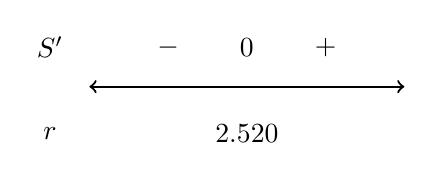
\begin{tikzpicture}[baseline=(current bounding box.center)]
            \draw[<->, thick] (0,0) -- (4,0);

            \node at (2,-0.6) {2.520};
            \node at (-0.5, -0.6) {$r$};

            \node at (1,0.5) {$-$};
            \node at (2,0.5) {$0$};
            \node at (3,0.5) {$+$};
            \node at (-0.5, 0.5) {$S'$};
        \end{tikzpicture}
    \end{center} \vspace{11pt}
    Because the derivative changes from negative to positive, we know that 2.5198 is a minimum. We can plug it back into our surface area equation to find our minimum surface area. \begin{align*}
        & S(2.5198) = 2\pi(2.5198)^2 + \dfrac{64\pi}{2.5198} \\[11pt]
        & S(2.5198) = 119.687 \si{in^2}
    \end{align*}
    Therefore, the minimum surface area of the cola can is $\boxed{119.687 \si{in^2}}$.
\end{tcolorbox}

A related rates problem is characterized by various measurements that are changing \textbf{in relation to each other}. The variables are still related to each other through a geometric or physical relationship. The key difference from other differentiation problems is that we differentiate implicitly with respect to time, rather than a variable like $x$. In other words, 

\begin{center}  
    \fbox{\fbox{\begin{minipage}{0.96 \textwidth}
        \begin{align*}
            & \text{Optimization Problems:} && \text{Apply } \diff \\[11pt]
            & \text{Related Rates Problems:} && \text{Apply } \dfrac{d}{dt} \\
        \end{align*}
    \end{minipage}}}
\end{center}

Now, let's take a look at this different (related rates) cola problem.

\begin{tcolorbox}[example]
    \textbf{Ex 1.8.2: } The volume of a cylindrical cola can is $32\pi \si{in^3}$. The height of the can is changing at $\dfrac{1}{4} \si{in \per sec} \forcespace$. If the radius changes at the same time so as to maintain the volume, how fast is the radius shrinking when the can is $4$ inches tall? 
\end{tcolorbox} 
\begin{tcolorbox}[solution]
    \textbf{Sol 1.8.2: } \begin{align*}
        & V = \pi r^2h = 32\pi \\[11pt]
        & h = \dfrac{32}{r^2} \\[11pt]
        & \tdiff\left[h = \dfrac{32}{r^2}\right] \\[11pt]
        & \dfrac{dh}{dt} = -\dfrac{64}{r^2}\left(\dfrac{dr}{dt}\right)
    \end{align*}
    Now that we have a method to find what we are looking for, $\dfrac{dr}{dt}$, let's substitute in the values that we are given in the problem. \begin{align*}
        & h = 4 \rightarrow \dfrac{32}{r^2} = 4 \rightarrow r^2 = 8 \\[11pt]
        & \dfrac{1}{4} = -\dfrac{64}{8}\left(\dfrac{dr}{dt}\right) \\[11pt]
        & \dfrac{dr}{dt} = \boxed{-\dfrac{1}{32} \si{in \per sec}}
    \end{align*}
\end{tcolorbox}

As we can see, many of the steps that we take in the related rates cola problem is similar to those of the optimization cola problem. 

\textbf{Process For Related Rates Problems} \par

\begin{enumerate}[label=\arabic*.]
    \item Draw a visual for the problem. 
    \item Label the visual with what is given and what is being asked. 
    \begin{enumerate}[label=\alph*.]
        \item Use variables for any quantities that are \textbf{changing}. 
        \item Pay particular attention to the units.
    \end{enumerate}
    \item Determine the equation(s) that relate the variables to each other.
    \begin{enumerate}[label=\alph*.]
        \item Decide which equation will be differentiated.
        \item If there is a product of two variables, eliminate the product by either multiplying the equation out or substituting a secondary equation.
    \end{enumerate}
    \item \textbf{Differentiate in terms of time!} This is the key step.
    \begin{enumerate}[label=\alph*.]
        \item Do not forget implicit fractions.
    \end{enumerate}
    \item Substitute the given information and solve for the missing variable.
    \item Reread the problem and make sure to answer the question that was asked.
\end{enumerate} \vspace{11pt}

A classic related rates problem is the falling ladder. 

\begin{tcolorbox}[example]
    \textbf{Ex 1.8.3: } A $13$-foot ladder is leaning against a wall. The bottom of the ladder slides away from the wall at $4 \si{ft \per sec}$. How fast is the top of the ladder moving down the wall when the ladder is $5$ feet from the wall? \\[11pt]

    \begin{center}
        \begin{tikzpicture}[tdplot_main_coords, scale=1.25]

            % Wall (x-z plane at y=0)
            \fill[gray!5, opacity=0.8] (0,0,0) -- (0,4.5,0) -- (-4.5,4.5,0) -- (-4.5,0,0) -- cycle;

            % Floor (x-y plane at z=0)
            \fill[gray!10, opacity=0.7] (0,0,0) -- (-4.5,0,0) -- (-4.5,0,4.5) -- (0,0,4.5) -- cycle;

            % Axes
            \draw[->] (0,0,0) -- (-5,0,0) node[anchor=south]{$z$};
            \draw[->] (0,0,0) -- (0,0,5) node[anchor=south]{$y$ (ladder height)};
            \draw[->] (0,0,0) -- (0,5,0) node[anchor=west]{$x$ (ladder base)};

            % Ladder
            \draw[very thick, red] (0,0,4) -- (0,1.667,0);
            \draw[very thick, red] (-0.5,0,4) -- (-0.5,1.667,0) node[pos=0.35, above right, sloped] {Ladder};
            \foreach \i in {1,...,7} {
                \draw[very thick, red] ({0}, {0.208*\i}, {4 - 0.5*\i}) -- ({-0.5}, {0.208*\i}, {4 - 0.5*\i});
            }

            % Labels
            \node at (0,2.3,1.5) [red] {$\ell = 13$};
        
        \end{tikzpicture}
    \end{center}           
\end{tcolorbox}
\begin{tcolorbox}[solution]
    \textbf{Sol 1.8.3: } As can be seen in the visual, the height of the top of the ladder and the distance the bottom of the ladder is from the wall is related through the Pythagorean theorem. Both are variables, because the ladder is moving. \begin{align*}
        x^2 + y^2 = 13^2
    \end{align*}
    We are given the information that the bottom of the ladder slides away from the wall at $4 \si{ft \per sec}$. Therefore, we can say that our $\dfrac{dx}{dt} \forcespace = 4$. To find $\dfrac{dy}{dt}$, we differentiate $x^2 + y^2 = 13^2$ to get \begin{align*}
        2x\dfrac{dx}{dt} + 2y\dfrac{dy}{dt} = 0
    \end{align*}
    Although this may seem like a complex four equation variable, we already know $x$ and $\dfrac{dx}{dt} \forcespace$. We also can determine that $y = 12$ by the Pythagorean theorem. So, \begin{align*}
        & 2x\dfrac{dx}{dt} + 2y\dfrac{dy}{dt} = 0 \\[11pt]
        & 2(5)(4) + 2(12)\dfrac{dy}{dt} = 0 \\[11pt]
        & \dfrac{dy}{dt} = \boxed{-\dfrac{5}{3} \si{ft \per sec}}
    \end{align*}
    It should make sense that $\dfrac{dy}{dt}$ is negative because the top of the ladder is sliding down.
\end{tcolorbox}

Below are some of the equations you should know for the AP exam: \par

\begin{center}  
    \fbox{\fbox{\begin{minipage}{0.96 \textwidth}
        \vspace{11pt}
        \begin{center}
            \textbf{Common Formulas For Optimization/Related Rates Problems} \\[11pt]
            \textbf{Pythagorean Theorem} \begin{align*}
                x^2 + y^2 = r^2
            \end{align*} 
            \textbf{Area Formulas} \begin{align*}
                & \text{Circle: } A = \pi r^2 && \text{Rectangle: } A = lw \\[11pt]
                & \text{Triangle: } A = \dfrac{1}{2}bh && \text{Trapezoid: } A = \dfrac{1}{2}h\left(b_1 + b_2\right)
            \end{align*}
            \textbf{Volume Formulas} \begin{align*}
                & \text{Sphere: } V = \dfrac{4}{3}\pi && \text{Right Prism: } V = Bh &&& \text{Cylinder: } V = \pi r^2h \\[11pt]
                & \text{Cone: } V = \dfrac{1}{3}\pi r^2h && \text{Right Pyramid: } V = \dfrac{1}{3}Bh &&& \text{*Washer: } V = \pi(R^2 - r^2)h
            \end{align*}
            \textbf{Surface Area Formulas} \begin{align*}
                & \text{Sphere: } S = 4\pi r^2 && \text{Cylinder: } S = 2\pi r^2 + 2\pi rh \\[11pt]
                & \text{Cone: } S = \pi r^2 + \pi rl && \text{*Right Prism: } S = 2B + Ph \\[11pt]
            \end{align*}
            \footnotesize{N.B. The two equations with asterisks are less commonly used.}
        \end{center} 
        \vspace{11pt}
    \end{minipage}}}
\end{center}

Another common related rates problem is where a tank of a particular shape is filling or draining. \par

\begin{tcolorbox}[example]
    \textbf{Ex 1.8.4: } A tank shaped like an inverted cone $8$ feet in height and with a base diameter of $8$ feet is filling at a rate of $10 \si{ft^3 \per min}$. How fast is the height changing when the water is $6$ feet deep? \\[11pt]

    \begin{center}
        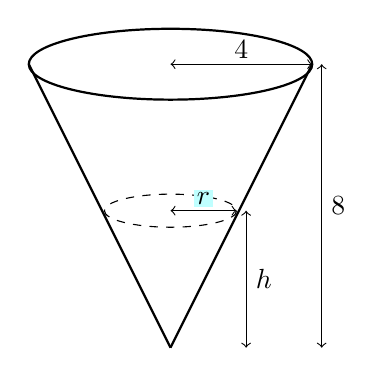
\begin{tikzpicture}[scale=0.6]
            \draw[thick] (-3,0) arc[start angle=180,end angle=540,x radius=3cm,y radius=0.75cm];

            \draw[thick] (-3,0) -- (0,-6);
            \draw[thick] (3,0) -- (0,-6);
            \draw[dashed] (-1.4,-3.1) arc[start angle=180,end angle=540,x radius=1.4cm,y radius=0.35cm];

            \draw[<->] (0, -3.1) -- (1.4, -3.1) node[midway, above, yshift=1pt, fill=Cyan!25, inner sep=1pt] {$r$};
            \draw[<->] (1.6, -3.1) -- (1.6, -6) node[midway, right] {$h$};
            \draw[<->] (0, 0) -- (3, 0) node[midway, above, yshift=-1.5pt] {$4$};
            \draw[<->] (3.2, 0) -- (3.2, -6) node[midway, right] {$8$};

        \end{tikzpicture}
    \end{center}

\end{tcolorbox}
\begin{tcolorbox}[solution]
    \textbf{Sol 1.8.4: } The units on the rate of change tell us that this is a change in volume, or $\dfrac{dV}{dt}$. Therefore, we use the equation \begin{align*}
        V = \dfrac{1}{3}\pi r^2h
    \end{align*}
    But, there are too many variables in this equation to differentiate as it stands. Since the rate of the change of the height---$\dfrac{dh}{dt} \forcespace$---is what we are looking for, we can eliminate $r$ from the equation. By similar triangles, we have \begin{align*}
        & \dfrac{r}{h} = \dfrac{4}{8} \\[11pt]
        & r = \dfrac{1}{2}h
    \end{align*}
    Substitution gives us a volume equation in terms of only height. \begin{align*}
        & V = \dfrac{1}{3}\pi\left(\dfrac{1}{2}h\right)^2h \\[11pt]
        & V = \dfrac{\pi}{12}h^3
    \end{align*}
    Differentiate and plug in our given values to solve for $\dfrac{dh}{dt}$. \begin{align*}
        & V = \dfrac{\pi}{12}h^3 \\[11pt]
        & \dfrac{dV}{dt} = \dfrac{\pi}{4}h^2\dfrac{dh}{dt} \\[11pt]
        & 10 = \dfrac{\pi}{4}(6)^2\dfrac{dh}{dt} \\[11pt]
        & \dfrac{dh}{dt} = \boxed{\dfrac{10}{9\pi} \si{ft \per min}}
    \end{align*}
\end{tcolorbox} \vspace{11pt}

\begin{tcolorbox}[example]
    \textbf{Ex 1.8.5: } Two cars approach an intersection, one traveling south at $20$ miles per hour and the other traveling west at $30$ miles per hour. How fast is the direct distance between them decreasing when the westbound car is $0.6$ miles and the southbound car is $0.8$ miles away from the intersection? \\[11pt]

    \begin{center}
        \begin{tikzpicture}[scale=0.5]
            
            \draw[arrow] (0, 0) -- (0, -8) node[midway, left, xshift=-11pt] {$y$};
            \draw[arrow] (6, -8) -- (0, -8) node[midway, below] {$x$};
            \draw[dashed] (0, 0) -- (6, -8) node[midway, above] {$r$};

            \fill[WildStrawberry!80] (-0.38, 0.38) -- (0.38, 0.38) -- (0.38, -0.75) -- (-0.38, -0.75) -- cycle;
            \fill[Blue!60] (5.25, -7.68) -- (6.38, -7.68) -- (6.38, -8.38) -- (5.25, -8.38) -- cycle;
            
        \end{tikzpicture}
    \end{center}
\end{tcolorbox}
\begin{tcolorbox}[solution]
    \textbf{Sol 1.8.5: } As we can see in the picture, the distance between the two cars are related by the Pythagorean theorem. \begin{align*}
        x^2 + y^2 = r^2
    \end{align*}
    We know several pieces of information. The southbound car is moving at $20$ miles per hour; i.e. $\dfrac{dy}{dt} = -20$. By similar logic, we can deduce each of the following: \begin{align*}
        & \dfrac{dy}{dt} = -20 && \dfrac{dx}{dt} = -30 \\[11pt]
        & y = 0.8 && x = 0.6
    \end{align*}
    And, by the Pythagorean Theorem, $r = 1$. Now we take the derivative of the Pythagorean theorem to get \begin{align*}
        2x\dfrac{dx}{dt} + 2y\dfrac{dy}{dt} = 2r\dfrac{dr}{dt}
    \end{align*}
    This is essentially an equation in six variables. But, we know five of those variables, so let's substitute and solve. \begin{align*}
        & 2(0.8)(-30) + (2)(0.6)(-20) = 2(1.0)\dfrac{dr}{dt} \\[11pt]
        & \dfrac{dr}{dt} = \boxed{-36 \si{mph}}
    \end{align*}
    It should make sense that $\dfrac{dr}{dt} \forcespace$ is negative since the two cars are approaching one another. The units also make sense: since $r$ is in miles and $h$ is in hours, the final units should be miles per hour.
\end{tcolorbox}

\begin{tcolorbox}[default]
    \begin{center}
        \textbf{Strategy For Related Rates Problems} \\[22pt]
    \end{center}
    \begin{center}
        \begin{tikzpicture}[node distance=2cm]
            
            \node (read) [startstop]
                {Read the problem and draw a visual.};
            \node (choose) [decision, below of=read, yshift=-1cm]
                {Choose a place to start.};
            \node (identify_c) [process, below of=choose, yshift=-1cm, text width=3.5cm]
                {Identify the constants given in the problem. \textbf{Use the units to decide.}};
            \node (identify_v) [process, left of=identify_c, text width=3.5cm, xshift=-3cm]
                {Identify the variables in the problem.};
            \node (decide) [process, right of=identify_c, text width=3.5cm, xshift=3cm]
                {Decide on the equation for the relationship between the variables};
            \node (undifferentiated) [process, below of=identify_c, xshift=-3.75cm, yshift=-1cm, text width=6cm]
                {Use the undifferentiated equation(s) to find any other missing constant(s)};
            \node (two_v) [process, below of=identify_c, xshift=3.75cm, yshift=-1cm, text width=6cm]
                {If there are more than two variables, substitute to eliminate an unnecessary variable.};
            \node (differentiate) [process, below of=two_v, text width=6cm, yshift=-0.25cm, xshift=-3.75cm]
                {Differentiate in terms of time.};
            \node (substitute) [process, below of=differentiate]
                {Substitute the constants into the differentiated equation.};
            \node (solve) [process, below of=substitute]
                {Solve for the missing variable};
            \node (reread) [startstop, below of=solve, align=center]
                {Reread the problem and answer the question that was asked. \\ \textbf{Don't forget the units}};
            
            \draw [arrow] (read) -- (choose);
            \draw [arrow] (choose.west) -| (identify_v.north);
            \draw [arrow] (choose) -- (identify_c);
            \draw [arrow] (choose.east) -| (decide.north);
            \draw [arrow] (identify_v) -- (undifferentiated);
            \draw [arrow] (identify_c) -- (undifferentiated);
            \draw [arrow] (decide) -- (two_v);
            \draw [arrow] (two_v) |- (differentiate.east);
            \draw [arrow] (undifferentiated.south) |- (differentiate.west);
            \draw [arrow] (differentiate) -- (substitute);
            \draw [arrow] (substitute) -- (solve);
            \draw [arrow] (solve) -- (reread);
        \end{tikzpicture}
    \end{center}
\end{tcolorbox}

\newpage

\textbf{\large{1.8 Free Response Homework}}

\onequestion{1. Two boats leave an island at the same time, one heading north and one heading east. The northbound boat is moving at $12 \si{mph}$ and the eastbound boat is moving at $5 \si{mph}$. At $t = 0.2$ hours, the northbound boat is $1.4$ miles away from the island and the eastbound boat is $1$ mile away from the island.}
\begin{enumerate}[label=\hspace{11pt}(\alph*), align=left, leftmargin=*, labelsep=0.25em]
    \item Draw a picture of the situation at any time $t$.
    \item What variables are present in the problem?
    \item What known quantities are given? What quantities can be determined directly from the given information? And what is the unknown for which to solve?
    \item What equation(s) relates the quantities? Which one will be differentiated?
    \item How fast is the distance between the two ships decreasing at $t = 0.2$ hours?
\end{enumerate} \vspace{11pt}

\onequestion{2. A railroad track and a road cross at right angles. An observer stands on the road $70$ meters south of the intersection and watches an eastbound train traveling $60 \si{m \per sec}$.}
\begin{enumerate}[label=\hspace{11pt}(\alph*), align=left, leftmargin=*, labelsep=0.25em]
    \item Draw a picture of the situation at any time $t$.
    \item What variables are present in the problem?
    \item What known quantities are given? What quantities can be determined directly from the given information? And what is the unknown for which to solve?
    \item What equation(s) relates the quantities? Which one will be differentiated?
    \item At how many meters per second is the train moving away from the observer $4$ seconds after it passes the intersection?
\end{enumerate} \vspace{11pt}

\onequestion{3. A circular ink stain is spreading (i.e. the radius is changing) at half an inch per second.}
\begin{enumerate}[label=\hspace{11pt}(\alph*), align=left, leftmargin=*, labelsep=0.25em]
    \item Draw a picture of the situation at any time $t$.
    \item What variables are present in the problem?
    \item What known quantities are given? What quantities can be determined directly from the given information? And what is the unknown for which to solve?
    \item What equation(s) relates the quantities? Which one will be differentiated?
    \item How fast is the area changing when the stain has a $1$ inch diameter?
\end{enumerate} \vspace{11pt}

\onequestion{4. A screensaver has a rectangular logo that expands and contracts as it moves around the screen. The ratio of the sides stay constant, with the long side being $1.5$ times the short side. At a particular moment, the long side is $3 \si{cm}$, while the perimeter is changing by $0.25 \si{cm \per sec}$.}
\begin{enumerate}[label=\hspace{11pt}(\alph*), align=left, leftmargin=*, labelsep=0.25em]
    \item Draw a picture of the situation at any time $t$.
    \item What variables are present in the problem?
    \item What known quantities are given? What quantities can be determined directly from the given information? And what is the unknown for which to solve?
    \item What equation(s) relates the quantities? Which one will be differentiated?
    \item How fast is the area of the screensaver changing at the given moment?
\end{enumerate} \vspace{11pt}

\onequestion{5. Sand is being dumped onto a pile at $30\pi \si{ft \per min}$. The pile forms a cone with the height always equal to the base diameter.}
\begin{enumerate}[label=\hspace{11pt}(\alph*), align=left, leftmargin=*, labelsep=0.25em]
    \item Draw a picture of the situation at any time $t$.
    \item What variables are present in the problem?
    \item What known quantities are given? What quantities can be determined directly from the given information? And what is the unknown for which to solve?
    \item What equation(s) relates the quantities? Which one will be differentiated?
    \item How fast is the height changing when the pile is $5$ feet high?
\end{enumerate} \vspace{11pt}

\onequestion{6. A cylindrical oil tank of height $30'$ and radius $10'$ is leaking at a rate of $300 \si{ft^3 \per min}$.}
\begin{enumerate}[label=\hspace{11pt}(\alph*), align=left, leftmargin=*, labelsep=0.25em]
    \item Draw a picture of the situation at any time $t$.
    \item What variables are present in the problem?
    \item What known quantities are given? What quantities can be determined directly from the given information? And what is the unknown for which to solve?
    \item What equation(s) relates the quantities? Which one will be differentiated?
    \item How fast is the oil level dropping?
\end{enumerate} \vspace{11pt}

\onequestion{7. Water is leaking out of an inverted conical tank at a rate of $5000 \si{cm^3 \per min}$. The tank is $8 \si{m}$ tall and has a diameter of $4 \si{m}$.}
\begin{enumerate}[label=\hspace{11pt}(\alph*), align=left, leftmargin=*, labelsep=0.25em]
    \item Draw a picture of the situation at any time $t$.
    \item What variables are present in the problem?
    \item What known quantities are given? What quantities can be determined directly from the given information? And what is the unknown for which to solve?
    \item What equation(s) relates the quantities? Which one will be differentiated?
    \item Find the rate at which the height is decreasing when the water level is at $3 \si{m}$.
    \item Find the rate of change of the radius at the same instant as part (e).
\end{enumerate} \vspace{11pt}

\onequestion{8. Sand is dumped onto a pile at $30\pi \si{ft^3 \per min}$. The pile forms a cone with the height always equal to the base diameter. How fast is the base area changing when the pile is $10$ feet high?} \\[11pt]
\onequestion{9. A spherical balloon is being inflated so that its volume is increasing at a rate of $6 \si{ft^3 \per min}$. How fast is the radius changing when $r = 10 \si{ft}$?} \\[11pt]
\onequestion{10. The edge of a cube is expanding at a constant rate of $6$ inches per second. What is the rate of the change of the volume, in inches cubed per second, when the total surface area of the cube is $54 \si{in^2}$.} \\[11pt]
\onequestion{11. A $25$-foot tall ladder is leaning against a wall. The bottom of the ladder is pushed toward the wall at $5 \si{ft \per sec}$. How fast is the top of the ladder moving up the wall when it is $7$ feet up?} \\[11pt]
\begin{minipage}{0.5\textwidth}
    \onequestion{12. You are standing outside. A plane flies overhead, approaching you at constant altitude and a constant speed of $600$ miles per hour. When the plane flies over a house $13$ miles away from where you are standing, the angle of elevation is $0.647$ radians. How quickly is the direct (diagonal) distance between you and the plane changing at that moment?}
\end{minipage} \hfill \begin{minipage}{0.45\textwidth} \vspace{0pt}%
    \begin{center}
        \begin{tikzpicture}[scale=0.93]
            \draw[thick] (0, 0) -- (5, 0);
            \draw[dashed, thick] (5, 0) -- (5, 2.2);
            \draw[dashed, thick] (5, 2.2) -- (0, 0);
            \draw[thick] (4.7, 0) -- (4.7, 0.3) -- (5, 0.3);
            \draw[arrow] (1.25, 0) arc[start angle=0, end angle=30, radius=1cm];

            \node at (1.45,0.3) {$\theta$};
            \node at (5, 2.5) {\includegraphics[width=2cm]{\graphicsdir Chapter 1 Graphics/1.8-Graphic1.png}};
            \node at (-0.5, 0) {\includegraphics[width=0.75cm]{\graphicsdir Chapter 1 Graphics/1.8-Graphic2.png}};
        \end{tikzpicture}
    \end{center}
\end{minipage} \\[11pt]
\onequestion{13. The altitude of a triangle is increasing at a rate of $2 \si{cm \per sec}$ at the same time that the area of the triangle is increasing at a rate of $5 \si{cm^2 \per sec}$. At what rate is the base increasing when the altitude is $12 \si{cm}$ and the area is $144 \si{cm^2}$?} \\[11pt]
\onequestion{14. Two cars start moving away from the same point. One travels south at $60 \si{mph}$, and the other travels west at $25 \si{mph}$. At what rate is the distance between the cars increasing two hours later?} \\[11pt]
\onequestion{15. According to Boyle's Law, gas pressure varies directly with temperature and inversely with volume, as described by the following equation: \begin{align*}
    P = \dfrac{kT}{V}
\end{align*}
Suppose that the temperature is held constant while the pressure increases at at $20 \si{kPa \per min}$. What is the rate of change of the volume when the volume is $600 \si{in^3}$ and the pressure is $150 \si{kPa}$?} \\[11pt]
\onequestion{16. The Adiabatic Law for expansion of air can be represented with the equation \begin{align*}
    P \cdot V^{1.4} = \dfrac{4}{81},
\end{align*} where $P$ represents pressure and $V$ represents volume. If, at a specific instant, $P = 108 \si{lb \per in^2}$ and is increasing at $27 \si{lb \per in^2}$ per second, what is the rate of change of the volume?} 

\onequestion{17. Person $A$ is $220$ feet north of an intersection and walking toward it at $10 \si{ft \per sec}$. Person $B$ starts at the intersection and walks east at $5 \si{ft \per sec}$.} \\[11pt]
\begin{minipage}{0.49\textwidth} 
    \vspace{-16.5pt} %Countercorrection
    \begin{center}
        \begin{tikzpicture}[scale=0.55]
            \draw[thick] (0, 0) -- (2, 0) -- (2, 5);
            \draw[thick] (4, 5) -- (4, 0) -- (10, 0);
            \draw[thick] (0, -2) -- (2, -2) -- (2, -5);
            \draw[thick] (4, -5) -- (4, -2) -- (10, -2);

            \node at (3, 4.5) {$A$};
            \node at (3, -1) {$B$};
            \draw[arrow] (3, 4) -- (3, 1);
            \draw[arrow] (3.5, -1) -- (6.5, -1);
        \end{tikzpicture}
    \end{center}
\end{minipage} \hfill \begin{minipage}{0.5\textwidth} \vspace{0pt}%
    \begin{enumerate}[label=\hspace{11pt}(\alph*), align=left, leftmargin=*, labelsep=0.25em, itemsep=1em]
        \item At $t = 10$ seconds, how far is each person from the intersection? 
        \item At $t = 10$ seconds, how far apart are the two people? 
        \item How fast is the distance between the two people changing at $t = 10$ seconds? 
        \item At time $t = 10$ seconds, if person $A$ looks at person $B$, how fast is the angle between person $A$'s line of sight to person $B$ and the eastward direction changing? 
    \end{enumerate} \vspace{11pt}
\end{minipage} 

\onequestion{18. A fire truck is parked $7$ feet away from the base of a building and its ladder is extended to the top of the building. The ladder retracts at a rate of $0.5$ feet per second, while the angle of the ladder changes such that the bucket at the end of the ladder comes down vertically.} \\[11pt]
\begin{minipage}{0.49\textwidth}
    \vspace{-16.5pt} %Countercorrection
    \begin{center}
        \begin{tikzpicture}[scale=0.8]
            \draw[thick] (0, 0) -- (2, 0) -- (2, 7) -- (0, 7) -- cycle;
            \fill[Gray!40] (0, 0) -- (2, 0) -- (2, 7) -- (0, 7) -- cycle;
            \draw[thick] (2, 0) -- (6, 0);
            \draw[thick] (6, 0) -- (2, 7) 
                node[midway, above, sloped] {Ladder};
            \draw[arrow] (5.4, 0) arc[start angle=170, end angle=135, radius=1cm];

            \node[rotate=90] at (1, 3.5) {Building};
            \node at (5.2, 0.4) {$\theta$};
            \node at (2, 7) {\includegraphics[width=1cm]{\graphicsdir Chapter 1 Graphics/1.8-Graphic3.png}};
            \node at (7, 0.5) {\includegraphics[width=1.6cm]{\graphicsdir Chapter 1 Graphics/1.8-Graphic4.png}};
        \end{tikzpicture}
    \end{center}
\end{minipage} \hfill \begin{minipage}{0.5\textwidth} \vspace{0pt}%
    \begin{enumerate}[label=\hspace{11pt}(\alph*), align=left, leftmargin=*, labelsep=0.25em, itemsep=1em]
        \item How far is the ladder extended when the bucket is $10$ feet above the ground?
        \item Find the rate at which the bucket is dropping vertically when the bucket is $10$ feet above the ground.
        \item What is the relationship between the angle $\theta$ and the height of the bucket? Find $\theta$, in radians, when the bucket is $10$ feet above the ground. 
        \item Find the rate, in radians per second, at which the angle the ladder forms with the ground is changing when the bucket is $10$ feet above the ground.
    \end{enumerate} \vspace{11pt}
\end{minipage}

\onequestion{19. A telephone crew is replacing a phone line from one telephone pole to the next. The line is on a spool on the back of a truck, and one end is attached to the top of a 25-foot pole. The vertical distance from the top of the pole to the level of the spool is 20 feet. The truck moves down the street at $20 \si{ft \per sec}$.} \\[11pt]
\begin{minipage}{0.49\textwidth}
    \vspace{-22pt} %Countercorrection
    \begin{center}
        \begin{tikzpicture}[scale=0.80]
            \draw[thick] (-0.25, 0) -- (0, 0) -- (0, 5) -- (-0.25, 5) -- cycle;
            \fill[Brown!50] (-0.25, 0) -- (0, 0) -- (0, 5) -- (-0.25, 5) -- cycle;
            \draw[thick] (0, 5) -- (5, 1);
            \draw[dashed] (0, 1) -- (5, 1);
            \draw[arrow] (0, 4.4) arc[start angle=280, end angle=315, radius=0.9cm];

            \draw[decorate, decoration={brace, mirror}, thick] 
                (-0.5, 5) -- (-0.5, 1) 
                node[midway, above, rotate=90, yshift=5pt] {$20 \si{ft}$};

            \node at (6.4, 0.6) {\includegraphics[width=2.5cm]{\graphicsdir Chapter 1 Graphics/1.8-Graphic5.png}};
            \node at (0.3, 4.1) {$\theta$};
        \end{tikzpicture}
    \end{center}
\end{minipage} \hfill \begin{minipage}{0.5\textwidth} \vspace{0pt}%
    \begin{enumerate}[label=\hspace{11pt}(\alph*), align=left, leftmargin=*, labelsep=0.25em, itemsep=1em]
        \item Find the length of line that has been rolled out when $t = 15$ seconds.
        \item Find the rate at which the telephone line is coming off the spool when the truck is $50$ feet from the pole.
        \item What is the relationship between the angle and the truck's distance from the pole? Find $\theta$, in radians, when the truck is $40$ feet from the pole.
        \item Find the rate, in radians per second, at which the angle the line forms with horizontal is changing when the truck is $40$ feet from the pole.
    \end{enumerate} \vspace{11pt}
\end{minipage}

\onequestion{20. At the end of the first season of the series \textit{Snowpiercer}, a second train (Big Alice) controlled by the industrialist Mr. Wilford came down another track to intercept and stop Snowpiercer. If the two train tracks meet at a $30^\circ$ then the Law of Cosines would apply such that $c^2 = a^2 + b^2 - 1.969ab$ as in the figure below. Snowpiercer is described as being two-and-a-half stories tall and $1,001$ cars long, with an average speed of $100 \si{km \per hour}$. Wilford's train Big Alice is much shorter, so it can average $120 \si{km \per hour}$.} \\[11pt]
\begin{minipage}{0.49\textwidth}
    \vspace{-11pt} %Countercorrection
    \begin{center}
        \begin{tikzpicture}[scale=0.50]
            \draw[arrow] (0, 0) -- (9.95, -1.95) 
                node[midway, above] {$a$};
            \draw[arrow] (2.5, -5) -- (9.95, -2.05)
                node[midway, below] {$b$};
            \draw[dashed, thick] (2.5, -5) -- (0, 0)
                node[midway, left, xshift=-5pt] {$c$};

            \node[circle, fill=black, inner sep=1.5pt, label={[yshift=-7.5pt, xshift=2.5pt]below:Intersection}] at (10,-2) {};
            \node[circle, fill=black, inner sep=1.5pt, label={above:Wilford's Train}] at (0, 0) {};
            \node[circle, fill=black, inner sep=1.5pt, label={below:Snowpiercer}] at (2.5, -5) {};
        \end{tikzpicture}
    \end{center}
\end{minipage} \hfill \begin{minipage}{0.5\textwidth} \vspace{0pt}%
    \begin{enumerate}[label=\hspace{11pt}(\alph*), align=left, leftmargin=*, labelsep=0.25em, itemsep=1em]
        \item If Snowpiercer is $38 \si{km}$ from the junction, how soon will it reach the junction?
        \item If Wilford’s train is $45 \si{km}$ from the junction, which train will reach the junction first?
        \item How fast is the distance $c$ between the two trains changing when Snowpiercer is $38 \si{km}$ from the junction and Big Alice is $45 \si{km}$ from the junction.
    \end{enumerate} \vspace{11pt}
\end{minipage}

\onequestion{21. The triangle-shaped swamp on Oak Island has been proven to have been manmade sometime around 1250 AD, possibly by the Knights Templar. It has been drained several times, revealing a stone-paved wharf and paths, an ancient clay mine, and the remains of a galleon which had been destroyed by fire and sunk in the swamp to conceal it. The triangle is roughly isosceles, with legs measuring $730$ feet and a base of $640$ feet. The apex (top angle) of the triangle measures $0.79$ radians.} \\[11pt]
\begin{minipage}{0.49\textwidth}
    \vspace{-11pt} %Countercorrection
    \includegraphics[width=\textwidth]{\graphicsdir Chapter 1 Graphics/1.8-Graphic6.png}
    \vspace{22pt}
    \begin{center}
        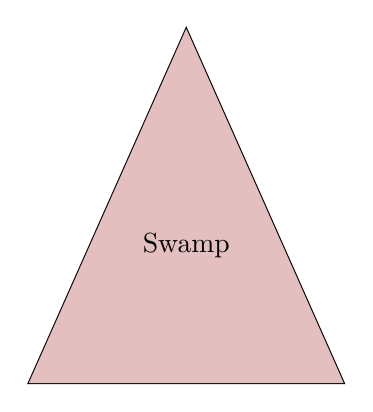
\begin{tikzpicture}[scale=0.5]
            \draw[thick] (0, 0) -- (8, 0) -- (4, 9) -- cycle;
            \fill[Brown!30] (0, 0) -- (8, 0) -- (4, 9) -- cycle; 

            \node at (4, 3.5) {Swamp};
        \end{tikzpicture}
    \end{center}
\end{minipage} \hfill \begin{minipage}{0.5\textwidth} \vspace{0pt}%
    \begin{enumerate}[label=\hspace{11pt}(\alph*), align=left, leftmargin=*, labelsep=0.25em, itemsep=1em]
        \item Based on the Law of Sines, the area of a triangle can be determined by the equation $Area = \dfrac{1}{2}ab\sin (C) \forcespace$, where $a$ and $b$ are the lengths of the legs and $\angle C$ is the measure of the angle in between the two legs. Find the surface area of the swamp before it was drained. Indicate the units.
        \item The length of third side of the triangle can be found using the Law of Cosine, $c^2 = a^2 + b^2 - 2ab\cos(C)$, where $c$ is the third side and $a$, $b$, and $\angle C$ are the same as those of part (a). How long is the third side when the legs are each $370$ feet?
        \item At $t = 24$ hours, the legs are $370$ feet and their rate of change is $-15.2 \si{ft \per hr}$. How fast is the third side of the triangle changing?
        \item Find the rate of change of the surface area. [Hint: Use the Law of Sines.] Indicate the units.
    \end{enumerate} \vspace{11pt}
\end{minipage}

\onequestion{22. A circle is inscribed in a square as shown. The circumference of the circle is increasing at a constant rate of $4$ inches per second. As the circle expands, the square expands to maintain the condition of tangency.}
\begin{center}
    \includegraphics[width=0.35\textwidth]{\graphicsdir Chapter 1 Graphics/1.8-Graphic7.png}
\end{center}
\begin{enumerate}[label=\hspace{11pt}(\alph*), align=left, leftmargin=*, labelsep=0.25em, itemsep=1em]
    \item Find the rate of change of the perimeter of the square.
    \item At the instant when the area of the circle is $16\pi$ square inches, find the rate at which the area \textit{between the square and the circle} is increasing.
\end{enumerate} \vspace{11pt}

\onequestion{23. An equilateral triangle is inscribed in a circle. The circle's circumference is expanding at $6\pi \si{in \per sec}$ and the triangle maintains the contact of its corners with the circle.}
\begin{center}
    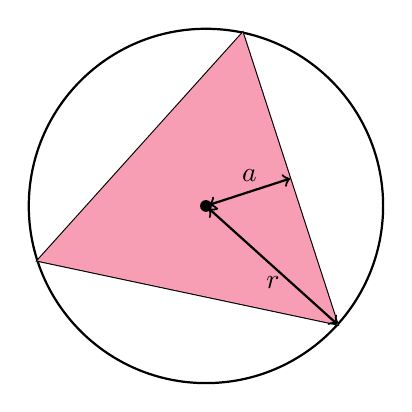
\begin{tikzpicture}[scale=0.75]
        \draw[thick] (0, 0) circle (3cm);
        \draw[thick] (0.623, 2.934) -- (-2.853, -0.927) -- (2.229, -2.007) -- cycle;
        \fill[WildStrawberry!40] (0.623, 2.934) -- (-2.853, -0.927) -- (2.229, -2.007) -- cycle;
        \draw[thick, <->] (0.05, 0.017) -- (1.427, 0.464)
            node[midway, above] {$a$};
        \draw[thick, <->] (0.05, -0.045) -- (2.22, -1.999)
            node[midway, below] {$r$};

        \node[circle, fill=black, inner sep=1.5pt] at (0, 0) {};
    \end{tikzpicture}
\end{center}
Given that the area of an equilateral triangle is equal to half the apothem $a$ times the perimeter $p$, find out how fast the area inside the circle but outside the triangle is expanding when the area of the circle is $64\pi \si{in}$. [Hint: Find $p$ and $a$ in terms of $r$.] \\[11pt]

\textbf{\large{1.8 Multiple Choice Homework}} \par

\begin{questions}
    \question The width of a square is increasing at a constant rate of $0.5 \si{cm \per sec}$. In terms of the perimeter $P$, what is the rate of change of the area of the square in centimeters squared per second? \\

    \begin{oneparchoices}
        \choice $-\dfrac{1}{2}P$
        \choice $-P$
        \choice $\dfrac{1}{4}P$
        \choice $\dfrac{1}{2}$
        \choice $P$
    \end{oneparchoices} \par \horizontalline

    \question When $x = 18$, the rate at which $y = \sqrt{0.5x}$ is increasing is $k$ times the rate at which $x$ is increasing. What is the value of $\dfrac{1}{k} \forcespace$? \\

    \begin{oneparchoices}
        \choice $\dfrac{1}{12}$
        \choice $\dfrac{1}{6}$
        \choice $1$
        \choice $6$
        \choice $12$
    \end{oneparchoices} \par \horizontalline

    \question The side of a cube is expanding at a constant rate of $6$ inches per second. What is the rate of change of the volume, in cubic inches per second, when the total surface area of the cube is $54 \si{in^2 \per sec}$? \\

    \begin{oneparchoices}
        \choice $324$
        \choice $108$
        \choice $18$
        \choice $162$
        \choice $54$
    \end{oneparchoices} \par \horizontalline

    \question If the volume of a cube is increasing at 20 cubic inches per second when each edge is $10$ inches long, how fast is the surface area increasing? \\

    \begin{oneparchoices}
        \choice $\dfrac{4}{3}$
        \choice $2$
        \choice $4$
        \choice $6$
        \choice $8$
    \end{oneparchoices} \par \horizontalline

    \question When the height of a cylinder is $12 \si{cm}$ and the radius is $4 \si{cm}$, the circumference is increasing at a rate of $\dfrac{\pi}{4} \forcespace$ \\

    \begin{oneparchoices}
        \choice $4\pi$
        \choice $12\pi$
        \choice $20\pi$
        \choice $80\pi$
        \choice $100\pi$
    \end{oneparchoices} \par \horizontalline

    \question At what approximate rate (in cubic meters per minute) is the volume of a sphere changing at the instant when the surface area is $3$ square meters and the radius is increasing at the rate of $\dfrac{1}{5} \forcespace$ meters per minute? \\

    \begin{oneparchoices}
        \choice $1.228$
        \choice $1.905$
        \choice $0.649$
        \choice $0.600$
        \choice $0.620$
    \end{oneparchoices} \par \horizontalline 

    \question The radius of a sphere is decreasing at a rate of $2$ centimeters per second. At the instant when the radius of the sphere is $3$ cm, what is the rate of change, in square centimeters per second, of the surface area of the sphere? [Hint: The surface area $S$ of a sphere with radius $r$ is $4\pi r^2$.] \\

    \begin{oneparchoices}
        \choice $-108\pi$
        \choice $-72\pi$
        \choice $-48\pi$
        \choice $-24\pi$
        \choice $-16\pi$
    \end{oneparchoices} \par \horizontalline

    \question Water is flowing into a spherical tank with a $6$-foot radius at the constant rate of $30\pi \si{ft^3 \per hour}$. When the water is $h$ feet deep, the volume of the water in the tank is given by the equation \begin{align*}
        V = \dfrac{\pi h^2}{3}(18 - h).
    \end{align*}
    What is the rate at which the depth of the water in the tank is increasing the moment when the water is $2$ feet deep? \\

    \begin{oneparchoices}
        \choice $0.5 \si{ft \per hour}$
        \choice $1.0 \si{ft \per hour}$
        \choice $1.5 \si{ft \per hour}$
        \choice $2.0 \si{ft \per hour}$
        \choice $2.5 \si{ft \per hour}$
    \end{oneparchoices} \par \horizontalline

    \question The radius of a circle is in increasing at a constant rate of $0.2$ meters per second. What is the rate of increase in the area of the circle at the instant when the circumference of the circle is $20\pi$ meters? \\

    \begin{oneparchoices}
        \choice $0.04\pi \si{m^2 \per sec}$
        \choice $0.4\pi \si{m^2 \per sec}$
        \choice $4\pi \si{m^2 \per sec}$
        \choice $40\pi \si{m^2 \per sec}$
        \choice $100\pi \si{m^2 \per sec}$
    \end{oneparchoices} \par \horizontalline

    \question If the rate of change of a number $x$ with respect to time $t$, is $x$, what is the rate of change of the reciprocal of the number when $x = -\dfrac{1}{4} \forcespace$? \\

    \begin{oneparchoices}
        \choice $-16$
        \choice $-4$
        \choice $-\dfrac{1}{48}$
        \choice $\dfrac{1}{48}$
        \choice $4$
    \end{oneparchoices} \par \horizontalline

    \question Gravel is being dumped from a conveyor belt at a rate of $35 \si{ft^3 \per min}$ and its coarseness is such that it forms a pile in the shape of a cone whose base diameter and height are always equal. How fast is the height of the pile increasing when the pile is $15 \si{ft}$ high? \\

    \begin{oneparchoices}
        \choice $0.27 \si{ft \per min}$
        \choice $1.24 \si{ft \per min}$
        \choice $0.14 \si{ft \per min}$
        \choice $0.20 \si{ft \per min}$
        \choice $0.60 \si{ft \per min}$
    \end{oneparchoices} \par \horizontalline

    \question Two cars start moving from the same point. One travels south at $28 \si{mi \per h}$ and the other travels west at 70 $\si{mi \per h}$. At what rate is the distance between the cars increasing $5$ hours later? \\

    \begin{oneparchoices}
        \choice $75.42 \si{mi \per h}$
        \choice $75.49 \si{mi \per h}$
        \choice $76.40 \si{mi \per h}$
        \choice $75.39 \si{mi \per h}$
        \choice $75.38 \si{mi \per h}$
    \end{oneparchoices} \par \horizontalline

    \question A Golden Rectangle is one where the ratio (called $\phi$) of the length of the short side $w$ to the long side $l$ is equal to the ratio of the long side to the sum of the two sides. In other words, $l = 1.618w$. If a Golden Rectangle changes such that $w$ is growing at $2 \si{in \per min}$, how fast is the area changing when $w$ is $5$ inches? \\

    \begin{oneparchoices}
        \choice $1.618 \si{in^2 \per min}$
        \choice $16.18 \si{in^2 \per min}$
        \choice $3.236 \si{in^2 \per min}$ \\[11pt]
        \makebox[0.23\textwidth] \choice $32.36 \si{in^2 \per min}$
        \makebox[0.23\textwidth] \choice $37.78 \si{in^2 \per min}$
    \end{oneparchoices} \par \horizontalline
\end{questions}